\chapter{Spatial Yule}

The understanding of cities is greatly intensified according to the growing amount of data and the toolboxes, including Geographical Information Systems, statistical physics, and stochastic processes. However, despite the wealth of pieces of information and tools, we still lack the systematic understanding of how cities emerge as a whole. 

We present a stochastic spatial growth model to address how cities emerge, grow and especially, compete over limited resource and space. The approach emphasizes the evolutionary trajectories of cities, which are influenced by the competition for redistributive resources in a given space affected by local and regional conditions (e.g., topography and industrial status, respectively). To model this spatial competition mechanism, our out-of-equilibrium growth model determines a fixed bound on global growth rates. Our model predicts two phases of urbanization: (a) free growth phase, and (b) resource constraint phase. In phase (a), the rank size and spatial density distributions of the model are consistent with empirical Zipf's and Clark's laws in urban sciences, indicating the realistic urbanization process has not yet reached bottlenecks of resources; When this bottleneck is reached, (b) captures the inevitability of various urban diseases, such as urban shrinkage in developed cities and the spatial relocation of developments. Our approach sheds light on analyzing urbanization process by pointing out early warnings and harms of environmental capacity.


\section{Backgrounds} 

How do cities co-evolve over limited resources and space? To improve the conceptional understanding of urbanization and landscape evolution under complex circumstances, we need to set up a collection of spatial growth models that give rules for individual citizens to derive macroscopic dynamical state of cities. Such models are powerful tools to understand urban growth dynamics~\cite{PhysRevX.4.011008, Li2017Simple, makse1995modelling, rybski2013distance, nanda2017spatial}. Theoretically, these models fill the gap between macroscopic patterns, such as socio-economic scalars and material properties, and microscopic dynamics, such as individual level interaction patterns; practically, these models investigate how different growth factors contribute to a city's emergence, and how these dynamics lead to the observed scaling laws~\cite{bettencourt2007growth,court2013origins,batty2008size,batty2019urbanscalinglaw}, fractality~\cite{batty1994fractal,batty2007cities}, and city size distributions (i.e., Zipf's law)~\cite{zipf1949human}. These models give quantitative references of urban growth trajectories broadly through urban morphology and spatial structures for urban planers and policy makers~\cite{anas1998urban}. The referred works have built natural paths for deriving macroscopic dynamical states from microscopic growth rules. Most of these approaches are based on the assumptions of homogeneous growth in Euclidean geometry. However, recent discoveries about complex spatial phenomena associated with realistic urban systems are better described using fractal or discrete geometry\cite{makse1995modelling,louf2014congestion,PhysRevE.58.7054}, which is more consistent with growth dynamics in disordered contexts and media. From an individual perspective, existing models cannot incorporate spatially heterogeneous social group structures, such as ages\cite{PhysRevE.93.012112} and limited work opportunities. This limitation calls for a model with simple mechanisms to include such information.

To capture the competitions for resources among cities, we develop a spatial growth model based on inconsistent space and memory-based growth dynamics. In this model, a subset of citizens, dominated by a total count of $N^*$ are referred as active population, representing the resources shared by the whole region. New cities spontaneously emerge over free space, and a city is defined as a continuous surface developed by the same emergence. Spatial sprawl and advancing urbanization are realized by the sequential settlement of new citizens. We claim that the location choice of each newly initiated citizen is regulated to be adjacent to the finite \textit{active population}, that are replacive under capacity. So a new initiation is also denoted as an \textit{introduction}. Such choices of newly introduction of citizens keeps spatial preferential attachment and competition at once. We show that beyond the desolated growth of each city, competitions introduced by spatial specialization and limited resources result in the vicissitudes of cities and urban shrinkage. Our model combines two themes that are relevant to many disciplines, including probability theory and ecology: The spatial preferential attachment mechanism~\cite{Li2017Simple} and the existence of environmental capacity under competition~\cite{gude2020bacterial,liu2019an}. 

% 刘老师意见:去掉On the first/second point On the first point, 
The first theme is spatial preferential attachment (or more generalized, the \textit{rich get richer} mechanism) that is well-observed in social systems, especially, where human settlements are clustered hence cities~\cite{marsili1998interacting}. Literature has discussed how urban features emerge from preferential attachment via interaction density~\cite{ccolak2016understanding,louf2014congestion,fujita1976spatial}, e.g., multiplicative or correlated percolation~\cite{makse1995modelling,PhysRevE.58.7054,rybski2013distance}, spatial networks~\cite{marsili1998interacting,court2013origins,Li2017Simple}, and utility maximization~\cite{PhysRevE.90.042815,axtell2001emergent}. Spatially, such mechanism leads to population clustering near every urban center. In this study, we adopt the spatial aspect from the idea of diffusion-limited aggregation~\cite{makse1995modelling, rybski2013distance, kleinberg2000navigation}, i.e., in each city, new comers settle near those active citizens.

%On the second point, 
Second, cities are systems with environmental capacity, e.g. the government's finance is supported by the city's pillar industries and that excessive employees do not guarantee a proportional urban output. Such observations are elaborated by finite technical demands and increasing infrastructural demands. In words, the involution of urbanization leads to decreased urban attractiveness~\cite{atkinson2012urban, girardin2009quantifying,gomez2018explaining,parris2003characterizing,batty2008size}, but however is poorly reflected in the referred works mostly base on certain equilibrium conditions or optimization aims~\cite{zipf1949human}. However, cities are inter-competitive and out-of-equilibrium to be consistent with the conditions needed for sustainability\cite{fujita1976spatial,louf2014congestion,ccolak2016understanding}. We therefore include rules for spatial exclusiveness and a bounded growth rate. Here, as also in non-spatial contexts~\cite{PhysRevE.55.R3817}, we intensified the restrictive settings for the inter-city competitions for active populations~\cite{batty2017urban}. We later prove that our space-relevant model extends the previous non-spatial predictions for city size distributions. These settings also result in realistic urban phenomena, such as ranking turnovers~\cite{gabaix2004evolution}, and urban shrinkage~\cite{haase2014conceptualizing}, that cannot be formulated by existing growth models.

\section{Spatial Yule Model}

Our model describes how cities emerge, grow, and compete over space, whose dynamics are determined mainly through three quantitative and spatial rules: 1) \textit{Active citizen rule}. We assume that during urban growth process, only `active' citizens attract new-comers to a nearby place in their city: $k$ and $N_i$ are the number of cities and active citizens in the $i$th city, respectively. 2) \textit{Memory kernel rule}. We take $\sum_{i} N_i \le N^*$ ($N^* \gg 1$) as the satiation condition, i.e., when the total population exceeds $N^*$, a new-comer would turn a random active dweller into inactive. In other words, the kernel includes up to $N^*$ active citizens in the whole region. This rule also introduces the age structures of the population, since each kernel-labeled person has an expected age presented later. 3) \emph{Spatial growth rule}. We assume the studied area is an $L\times L$ two-dimensional continuous space ($L\gg 1$) with a grid of cells and periodic boundary conditions, i.e., the locations of citizens are continuous, but the boundaries of cities are discrete by cells. A new city is seeded randomly over the region as a Poisson point process~\cite{miles1970homogeneous}, and it survives if its cell is not taken. Every new citizen settles at a constant distance $r\le 1$ and at a random angle $\theta$ from its introducer. Once a cell $c$ has held a citizen from the $i$th city, any citizens from another city $j$ ($j\ne i$) cannot introduce new-comers on cell $c$. Thus, cities are identified through their citizens' ancestral introducers and their geographical occupation of blocks. The spatial growth rule is parallel to Yule's settings for modeling the distribution of species per genus~\cite{yule1925ii} so our model could be regarded as a spatial Yule model with constraints (SYM). A sketch of the SYM is shown in Fig~\ref{sketchpic}.

Based on these rules, we can define the model with a set of two-phase master equations. Specifically, we assume that the probability of a population increase in city $i$ within the time interval $(t,t+dt)$ is $\beta_2N_idt$, where $\beta_2$ is the introduction rate of every active citizen; we also assume that new cities constantly emerge at a low rate of $\beta_1kdt$, proportional to the number of cities, where $\beta_1$ is the rate of new city generation. A city's generation is confirmed only if its location is an empty cell. The master equation can be written as \begin{align}\frac{\partial}{\partial t}N_i(t) =  \delta_{N_i(t)}\cdot k\beta_1+ (1-\delta_{N_i(t)})\cdot N_i\beta_2, \end{align} for the free growth phase, where urbanization is weakly dependent on space and resources $N^*$,
%[WHAT'S THE DEFINITION OF FREE GROWTH?], 
and \begin{align}
\frac{\partial}{dt} N_i(t) = \beta_2 N_i(t) -\delta_{\{\sum N_i = N^*\}}\cdot\notag \\ \left(\beta_1k(t) + (N^*-N_i(t))\beta_2 \right)
\end{align}
for the resource constraint phase, where the total resources $N^*$ are partitioned and new dwellers get resources only through redistribution. 
%[WHAT'S THE DEFINITION OF RESOURCE CONSTRAINT PHASE?]. 

\begin{figure}
	\centering
	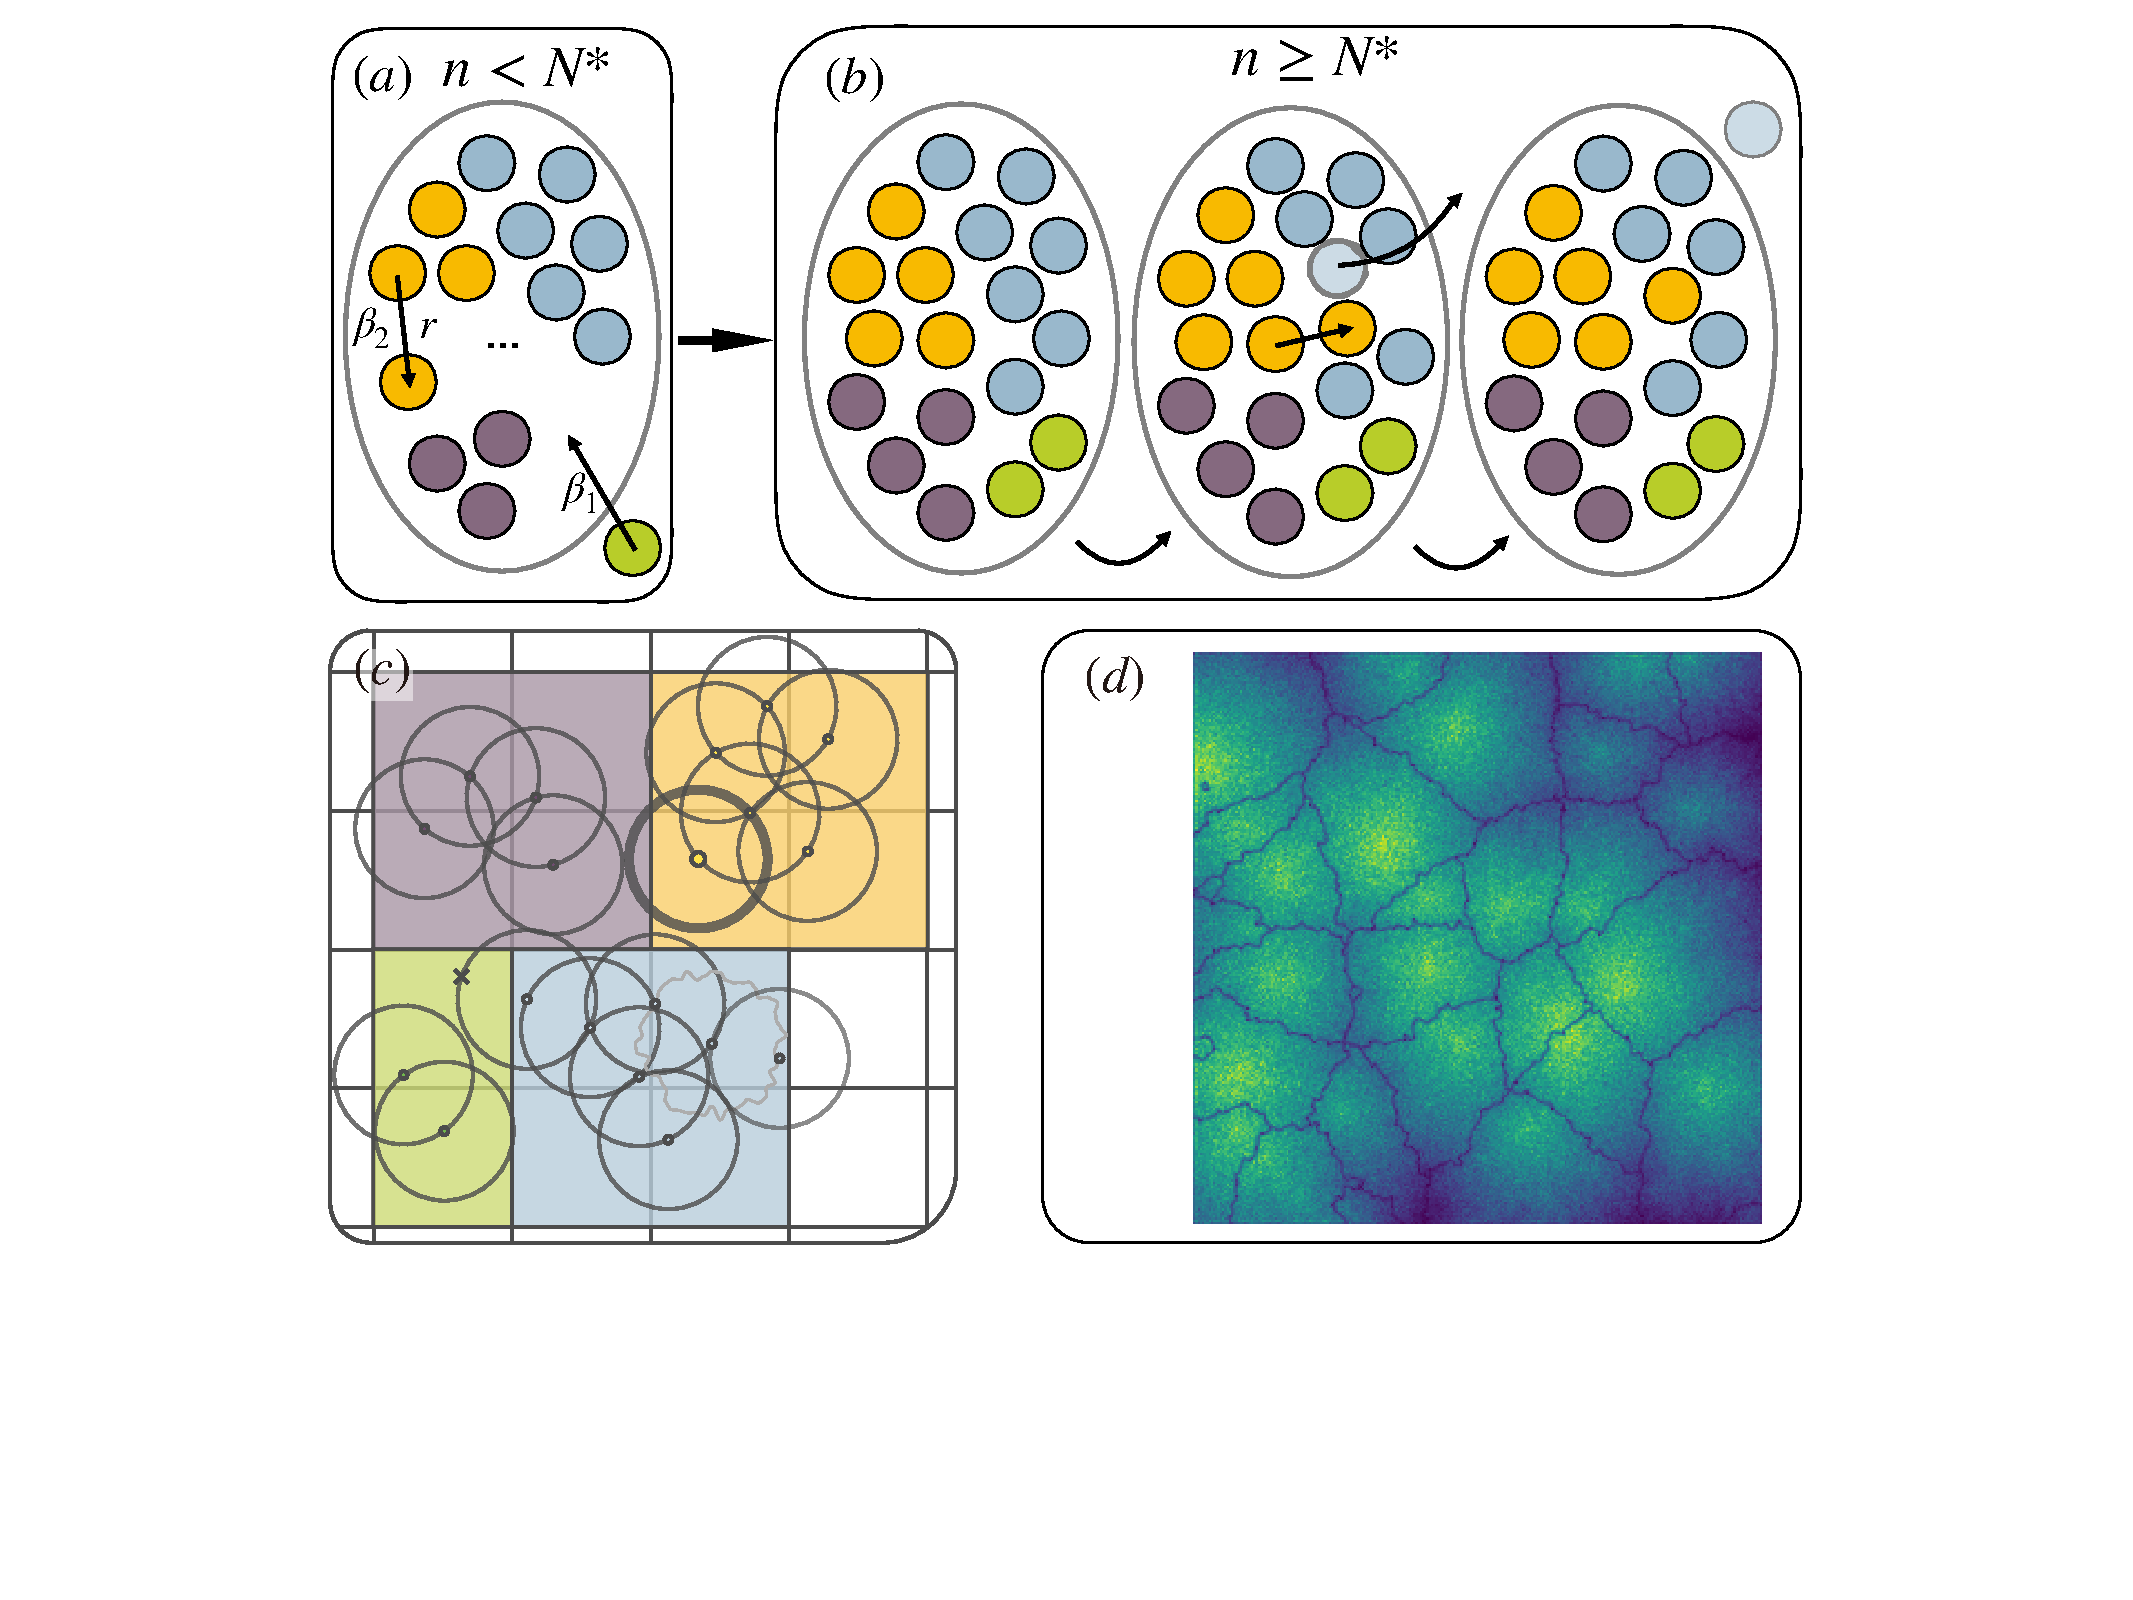
\includegraphics[width = 0.95\linewidth]{Pics/symsketch.pdf}
	\caption{\textbf{(a)} Status in the memory kernel at the free growth phase, i.e., the total population is less than $N^*$. Existing citizens introduce new dwellers at the rate $\beta_2$, while each existing city (noted by nodes in different colors) introduces new cities at the rate $\beta_1$. \textbf{(b)} When the memory kernel is fulfilled, every introduction of a new city or citizen leads to an ejection of an existing active citizen currently included in the memory kernel. \textbf{(c)} The spatial aspect of the model is that an offspring citizen's placement is at distance $r$ from the ancestral dweller. Also, when the kernel is filled, a new yellow node ejects an existing blue node and deprive her of the ability to introduce. \textbf{(d)} Simulated results for $L$, $r$, $\beta$ equal $256$, $0.5$, and $4$, respectively. We choose $\beta = 4$ to avoid confusion of too many cities shown. This is equivalent to a quarter of a $2L\times 2L$ simulation with $\beta = 1$.}
	\label{sketchpic}
\end{figure}

To summarize, the SYM can be regulated with three tunable parameters: the individual exploration distance $r$, the size of the memory kernel $N^*$, and the ratio $\beta:=\beta_2/\beta_1$. Though $\beta_1$ and $\beta_2$ actually represent generation speeds of cities and citizens, the model's dynamics and patterns are determined only by the relative growth rate $\beta$.

% 5. 模型需要哪些假设 6. 这些假设有什么理论和实证基础?
% [THE FOLLOWING PARA IS VERY CONFUNG. IF THIS IS ALSO RULES, YOU SHOULD PLACE THEM IN THE ABOVE PARA. IF THIS IS NOT, YOU SHOULD SPLIT THEM AND INSERT INTO THE PLACE THAT INTRODUCE PARAMETERS.] 
The model implies some simple assumptions. The first is that urban developments are density-driven. Literature has suggested that density-driven social ties and interactions are important drivers of the economies of scale~\cite{pan2013urban, girardin2009quantifying, batty1992form}. In the SYM, we further assume that only the density of the attractive population corresponds to urban developments. Such active population can be defined as the total number of employed or productive people. Secondly, to make an analytic framework, the growth dynamics are set to be homogeneous. The place choices for new comers are towards random directions; the rate of introductions and emergence are the same for every active citizen and every city. This diffusive setting of sequential settlements represents realistic urban growth~\cite{RevModPhys.87.925}. 

In the numerical experiments, which are elaborated in the Supplementary Material~\cite{SuppInfo}, the three parameters worth tuning are $\beta$, $r$, and $N^*$. $\beta$ contributes to the Zipfian coefficient and the turnover rate, defined as the frequency of other cities turning to be the largest~\cite{rooney2006structural}; $r$ refers to the fractality of urban areas and the time to fill the whole space; $N^*$ refers the severity of resource competition. 

% 7. 这个模型能推出哪些结论(1,2,3)。这些结论能如何被数据验证。
% \subsection{The free growth phase}

\subsection{The free growth phase}

SYM predicts three phases of regional growth of cities, distinguished by whether their resources and space have been fully occupied: the free growth phase, the economic constraint phase, and the spatial constraint phase. We focus on the first two phases, which correspond to regional resource. The evolution of the spatial constraint phase implies a fully urbanized region, which is unlikely to be seen in reality; we discuss the situation only in the Supplementary Material~\cite{SuppInfo}. In the free growth phase, cities grow isolatedly as new citizens being introduced into each of them over time, without being limited by resources and space. In this phase, SYM reformulates two important properties, stately (1) Zipf's law~\cite{gabaix1999zipf's} for rank size distribution of cities' population, and (2) Clark's law for exponential decay of urban density\cite{clark1951urban}. 

City populations typically decay proportionally to the inverse of their rank sizes~\cite{gabaix1999zipf's}. This is called Zipf's law of cities' population sizes, i.e., city populations are distribute as a power of ranks, $f_r(r)\sim r^{-(1+\eta)}$. It can be easily proved that $N_i(t)$ has a geometric distribution of $P(N_i(t)=n)=e^{-\beta_1t}(1-\exp(- {\beta_1} t))^{n-1}$~\cite{durrett1999essentials}. Combining which with the assumption that the number of cities will grow exponentially at rate $\beta_1$, if we randomly pick an existing city, the waiting time since its first appearance is exponential with parameter $\beta_1$. Thus, the distribution of a random city's population is 
\begin{align}
	f(n)=\frac{\Gamma(1+1/\beta)\Gamma(n)}{\beta\Gamma(n+1+1/\beta)}\approx Cn^{-1-1/\beta}, \ \text{as } n\to\infty,
\end{align}
where $\Gamma(\cdot)$ is the \textit{gamma} function. This equation implies a Zipfian relationship with $n(\text{rank})\sim {rank}^{-\beta}$. Noticing that $\beta$ takes its value from all positive real numbers in our model, we can derive arbitrary scaling behaviors by altering $\beta$. According to some studies~\cite{PhysRevLett.79.523}, the power law dependence of population frequency is $2.03\pm 0.05$ for the entire world, indicating that the average relative emerging rate of cities is around $1$. 

Varying $\beta$ allows considerations of study areas of different sizes. A small (large) $\beta$ indicates that the emergence of cities is fast (slow), corresponding to a large (smaller) study area. %[HOW ABOUT A LARGER BETA?] 
Thus, varying $\beta$ is parallel to investigating the spatial density of cities in an urban system. Some urban systems tend to form new cities to have sufficient infrastructures and less diversity of urban output~\cite{batty2008size} ($\beta > 1$) and some cities may go otherwise ($\beta< 1$). So the value $\beta$ actually reflects the intensity of regional population concentrations in large cities. The experiments have confirmed our analytic results for the free growth phase of SYM. %[I DON'T UNDERSTAND FROM `IT IS INTERESTING ... IN SYM. WHY THIS VALUE IS A REFECTION?] 
A simulated validation of these results is shown in Fig.~\ref{Fig2}. Notably, when $\beta$s are large ($>2$), the simulated Zipfian exponents are remarkably larger than their theoretical predictions. This is because the competition for space benefits small %[WHY LARGE SMALL CITIES?]
cities because of their higher percentage of edging cells, which is proved in the Supplementary Material~\cite{SuppInfo}. For systems of large $\beta$s for the cities at the same rank, however, the probability of the successful emergence of a new city decreases due to the relatively large area of existing cities. This exacerbates the concentration of active population in large cities.%% [UNCLEAR].
\begin{figure}[t]
	\centering
	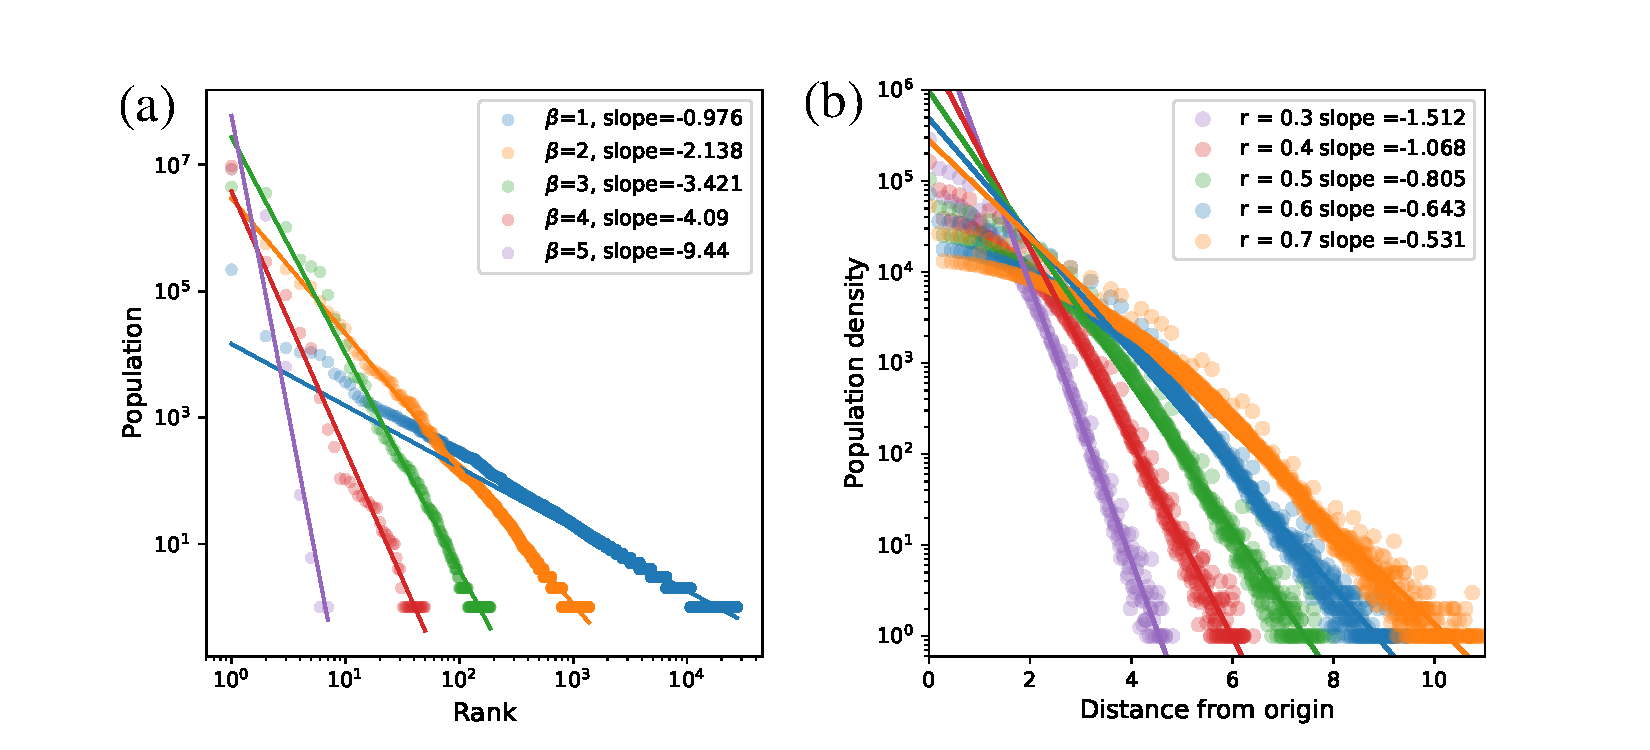
\includegraphics[width = .99\linewidth]{Pics/Zipf_Clark.pdf}
	\caption{\textbf{(a)} The distribution of population among cities. In the simulation, we take $N^* = 10^5$ and vary $\beta$s. A realistic Zipf coefficient is produced when $\beta\approx 1$. The theoretical predictions of the slopes are $-\beta$, and are well approximated when $\beta$ is small. A larger $\beta$ reduces the chance of later city's emergence. Thus, the spatial aspects of the SYM strengthen the inequality among sequential established cities. This result confirms that Zipf's law is valid for growing urban systems where all cities share the same growth rate. From the other master equation, we find that the Zipfian observation vanishes if total growing force is finite. \textbf{(b)} The population distribution as a function of distance from a district's center for different step lengths $r$. A larger $r$ stands for a more flattened urban sprawl. The vertical axis is logarithmically processed, which reveals that the spatial population density decays exponentially for each $r$.}
	\label{Fig2}
\end{figure}

%% Clark
% [WHAT'S THE LOGIC SENTENCE FOR THE FOLLOWING PARA? I.E., WHAT'S THE CONNECTION BETWEEN THE FOLLOWING TO ABOVE-MENTIONED THINGS?]
SYM also revisits Clark's law in urban studies~\cite{clark1951urban}. In SYM, population density evolves as a two-dimensional diffusion within a city\cite{doi:10.1137/0150099}, where we can focus the density's growth on each axis from the oldest citizens of a city. Let $\rho(d)$ denote the distance from the location of the active population density from a city center, and $t_n$ denote the time for the $n$'th citizen to be generated, we have 
\begin{align}
	\rho_{t_{n+1}}(d) = (\rho_{t_{n}}(d-r) + \rho_{t_{n}}(d+r) )/2.\label{loc_den}  
\end{align} By re-scaling time as $\tau_n = t_n\cdot (k\beta_1+N\beta_2)/T$, for a sufficiently large $T$, this equation results in an exponential decay of density
\begin{align}
	\rho(d)\sim e^{-\alpha d}\label{clark_eq}.
\end{align} A detailed proof is presented in the Supplementary Material~\cite{SuppInfo}. 

A direct implication of Clark's law is the strength of the competition at urban edges, which also influences the local Zipfian exponents. According to Clark's law, the population density is just a function of a city's age and the distance from urban center. Specifically, the density at the edges is important because it determines the competitive advantages for space. The population within an edge cell of city $j$ is estimated by $e^{(T-T_j)}\int_{d}^{d+1}\rho(r) dr/(2\pi d)$, where $T_j$ is the emerging time of city $j$. We also have the waiting time $T_{n+1}-T_{n}\sim 1/n$, and the total population approximation $e^{\beta_1+\beta_2}$, by combining which we derive the density of edging cells if time and the urban radius are given. Since a large urban center is more attractive, the population at the edge of large cities is actually smaller than that of minor cities. We validate our prediction with simulations, shown in Fig.~\ref{Fig2}. %[DON'T FOLLOW UP THIS PARA, WHY IT HERE, WHY IT IMPORTANT?] %We give a detailed derivation in Appendix B\ref{edge_comp}.
In addition, a larger $r$ will weaken the above prediction, as the settlements are more even, so a larger proportion of citizens lives at the edges. In reality, the metropolis areas over the world have very different densities. In SYM, $r$ corresponds to the sprawl of a city with given population. It can also be taken to study the proportion of a city's area in the studied region. On the other hand, it also controls the spatial limit of cities, given a competitionless population.

\subsection{The economic constraint phase}

The multi-perspective coincidence among the exponents derived in our model and those in the empirical evidence of population studies, which indicates that only two observation scales (city and citizen) lead to the behaviors of regional dynamics. This means that actual urban growth has not yet reached the constrained cases. However, preventive measures are still necessary. Thus, we adopt a general constraining parameter $N^*$ to further discuss the second phase of SYM, the economy constraint phase, in which the total population reaches $N^*$. Such a setting is an abstraction of many real-life rules set by global organizations, such as the allowable amount of carbon emissions or sustainable development projects. In each city, a proportion of the population is active. Here, $\sum_{i=1} N_i(t) = N^*$ for a sufficiently large $t$. If in a given period, minor cities generate more offspring than major ones, and the superiority of the remaining population within the memory kernel changes; a minor city's ranking will increase, as the growth rate of each city $i$ is actually $N_i\beta_2$. As for the dynamics within the memory kernel, in each city, $N_i$ acts as a random walk with absorption wall $0$, as no offspring will be expected if no nodes are left in the kernel. This result also works for single cell case within a city. We denote the population in cell $j$ of city $i$ as $m_{ij}$. According to the method in~\cite{durrett1999essentials}, we use a result for the branching process that a cell loses its vitality if the population falls below the threshold \begin{align}\rho_{threshold} = k/\beta.\end{align} This value shall be regarded as the sign for urban shrinkage, as the edging cells have a lower density according to equation~\ref{clark_eq} and thus have an exponentially higher probability of shrinking. In other words, urban shrinkage shall be reasoned by limited systematic resources. 

The kernel mechanism also plays a role at a cross-city scale: The preference for larger cities is fails more easily in a system with the memory kernel. Cities' competition for active citizens in SYM receives more than pure birth settings because the sum of the active population is given as $N^*$. In other words, the SYM system does not consider natural growth. To test this interpretation, we analyze the turnover rate, defined as the average frequency that the second largest city surpasses the largest in active population. We conduct numerical experiments, and receive power law dependence of the frequency of the simulation steps, as shown in Fig.~\ref{changerate}. Moreover, turnovers are more likely \textit{with} a memory kernel, meaning that turnover rate decay in probability slower if the system has constraints in resources. Another clear corollary is as a growing society (a society without a memory kernel) suffers less from inter-specific competition.

\begin{figure}
	\centering
	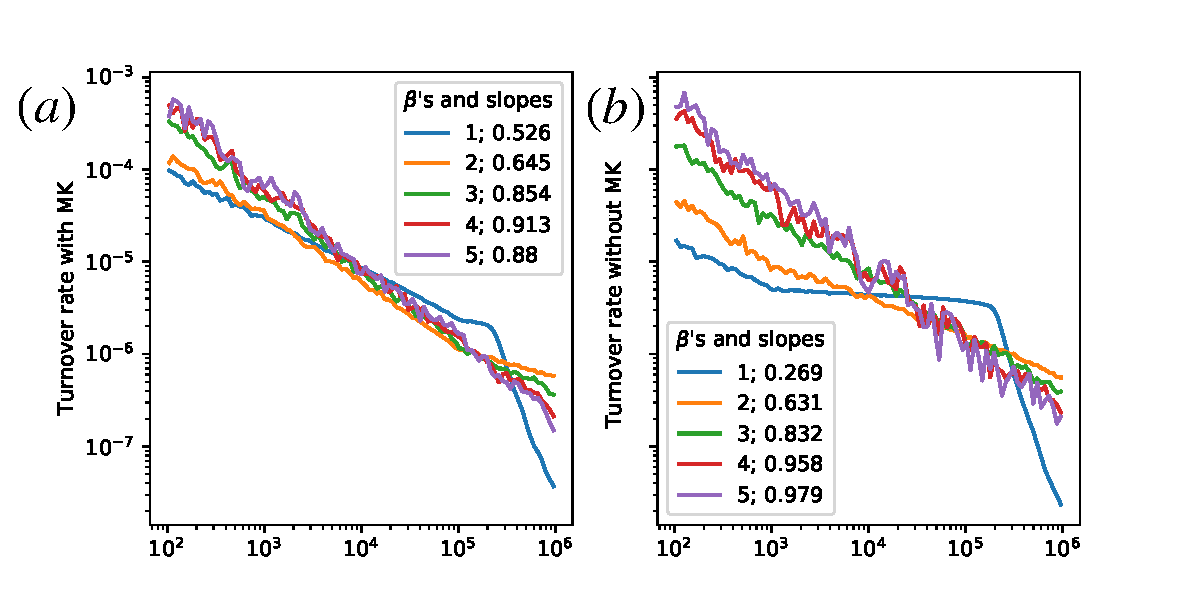
\includegraphics[width = 0.47\textwidth]{Pics/switchrate.pdf}
	\caption{The change rate statistics with \textbf{(a)} and without \textbf{(b)} a memory kernel. The kernel keeps turning over more often. With same $\beta$'s, a kernel-based SYM's decay in turnover rate is smaller. These results validate our prediction that with finite resource, advantages are more likely to be kept.}
	\label{changerate}
\end{figure}

The last property of SYM is the fractality of urban envelop, namely, the length of urban edges varies with the used measurement. Inspired by multi-player interactions in fractal financial market\cite{PhysRevE.65.037106}, we interpret that a fractal urban boundary is driven by the competition for land at cities' edges. In SYM, the uncertain competition for space lies in parameter $r$. A larger $r$ indicates greater randomness and creates an extra advantage for the smaller cities, resulting in a larger fractal dimension. We apply the box counting technique to calculate the fractal dimension of urban envelops, and receive a stable output of $d_f = 1.2\pm 0.05$ with $r = 0.5$, similar to empirical results~\cite{batty1992form}. We also find larger $d_f$s for a greater $r$. These results validate our hypothesis that fractal edges coexist with spatial competition. This result also confirms that SYM replicates an urban system.

% 总结我们这个模型的发现有哪些,为什么我们这个好。
\section{Chapter summary}

In recent years, we have witnessed the assumption of individual based models (IBMs) are insufficient for multi-phased urban growth dynamics. The simplest approach is to modify the classical dynamical systems, adjusting their growth potentials via empirically derived geographical heterogeneity in the IBMs. This approach is not satisfactory because it confounds attempts to extrapolate beyond the particular situations. An alternative, given the realistic basis of economic complexity and the central place theory, is to derive the causes of diversity; these measures are developed by abstracting the aggregated factors of production, and are predictive of future growth~\cite{Hidalgo10570}. It bridges a macroscopic dual to the IBMs. However, such an approach also has drawbacks for the economic complexity is even harder to monitor. 

In this work, we have attempted to bridge the gap between IBMs and macroscopic descriptions of urban systems. The memory kernel introduced here is a global condition clarifying how resources are shared by all cities: the governmental matching investment to allow the introduction of more new citizens. The restriction recipients at different scales of this mechanism exhibit fruitful characteristics: Microscopically, this is a realization of system-conditioned spatial preferential attachment. In the intermediate level of cities, the SYM introduces citizens' age structures and the accumulation of random shocks. The stationary age can be calculated as the average time for a new city to emerge with $(\beta_2 N^* + \beta_1 k)^{-1}$, which equals the average losing age of the whole kernel. This result gives an instruction of the length of a workable age in a given social urban system, elaborated in the Supplementary Material~\cite{SuppInfo}. The global trends predicted in our model are more random than those in non spatial and non-constraint models, allowing us to explain the vicissitudes of cities, and the changes in spatial structures in the post-urbanization phase. Despite the model's simplicity, it is still capable of reformulating major aspects of empirical observations of urban populations, including the Zipfian ranking of cities by population size and Clark's law for urban population density. The model also demonstrated the emergence of fractal urban edges. The generality of SYM can easily be embedded by spatial heterogeneous geographical circumstances, by adjusting the growth rate of each cell toward the product $m_{ij}\beta_2$, where $m_{ij}$ is the local characteristics.

% 不足
Although some results still need analytical proofs, this work is an essential step to strip out the power of urban dynamics. The model is non-commuting, but the community structure is naturally embedded. In further researches, we can extend the model by adding links, such as the volume of exploration and preferential return between cities~\cite{WANG2019121921}. The model can further be extended with a multi-dimensional memory kernel, allowing one citizen to be introduced if different factors~\cite{tokita2020social} (i.e., the existing citizens in different dimensions of the kernel) agree to allow her into the system.